\chapter{Propuesta del proyecto}
\label{chapter:proposed-method}

Este capítulo describe los componentes que integran el método propuesto, así
cómo la manera en cómo estos componentes proveen de apoyo al sistema final, este
capítulo está dividido en dos secciones la primera siendo la sección
\ref{section:used-method} en donde se explican los conceptos propuestos y
utilizados en el proyecto, esta sección se divide en varias subsecciones en
donde se explican partes de la propuesta y el cómo permitirán que el sistema
generado cumpla con los objetivos requeridos, la segunda sección
\ref{section:previous-proposed-methods} explica ideas y conceptos que se
propusieron a lo largo del desarrollo y el cómo estos ayudarían a mejorar el
sistema generado.

\section{Propuesta utilizada}
\label{section:used-method}

La propuesta final utilizada en el proyecto está basada en el uso de varias
técnicas para la generación de los compuestos y subsecuentemente los niveles
para el juego de Angry Birds, la base de todo el proyecto está en el uso de un
algoritmo genético para evolucionar los individuos, esto se explica más a
detalle en la sección \ref{subsection:generate-levels-using-GA}

\subsection{Generar compuestos de piezas base}
\label{subsection:generate-composites}

El videojuego de Angry Birds cuenta con un total de 11 diferentes tipos de
bloques, además de 2 grupos de objetos siendo estos cajas de explosivos y los
puercos que pueden ser colocados en el nivel, además de esto cuenta con
plataformas que pueden ser agregadas y rotadas para establecer plataformas en
donde colocar más bloques, de estos solo utilizaremos las 11 piezas básicas
mostradas en la Figura \ref{figure:game-basic-blocks} y los puercos para generar
niveles.

Las piezas básicas no pueden ser modificadas, tampoco es posible agregar nuevos
bloques al código debido a que la competencia solo utiliza las piezas regulares,
para poder librar esta restricción se generarán compuestos con las piezas base,
estos compuestos pueden estar formados de 1, 2 o más bloques básicos, estos
grupos se utilizarán para generar las estructuras que se colocaran en los niveles.

\begin{figure}
  \centering
  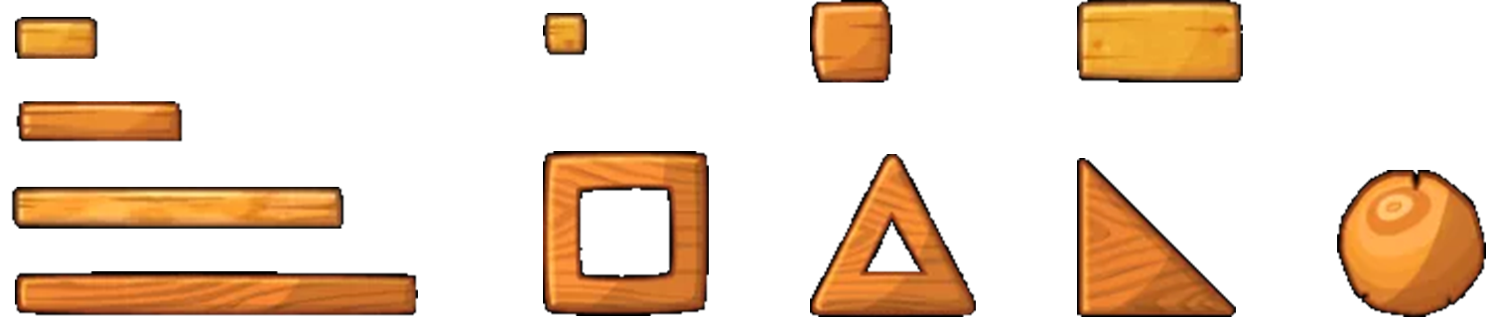
\includegraphics[width=1.0\textwidth]{img/list_pieces.png}
  \caption{Piezas básicas del juego angry birds}
  \label{figure:game-basic-blocks}
\end{figure}

La manera propuesta para generar estos conjuntos es mediante el uso de los
valores de alto y ancho de las piezas para poder definir los bordes de las
mismas, de esta manera al momento de querer unir dos o más piezas para formar un
conjunto la medida del conjunto se calculará buscando el punto más alto, más
bajo, así como las posiciones más a la derecha e izquierda teniendo ambas piezas
unidas, un ejemplo de la unión de cuatro piezas se muestra en la Figura
\ref{figure:bounding-box-calculation} en donde cuatro piezas se colocan una
sobre otra para formar un objeto cuadrado. Para poder agregar las piezas cómo
un conjunto se buscan los puntos más alejados, una vez que se ha calculado el
alto y ancho del conjunto se procede a encontrar el punto central del mismo,
desde este punto se calcula la distancia en \textit{x} y \textit{y} hacia los
centros de cada una de las piezas del conjunto, estos valores de centros se
agregan utilizando una estructura de diccionario para poder generar los objetos requeridos al
momento de crear a los individuos antes de iniciar las generaciones.

\begin{figure}
  \centering
  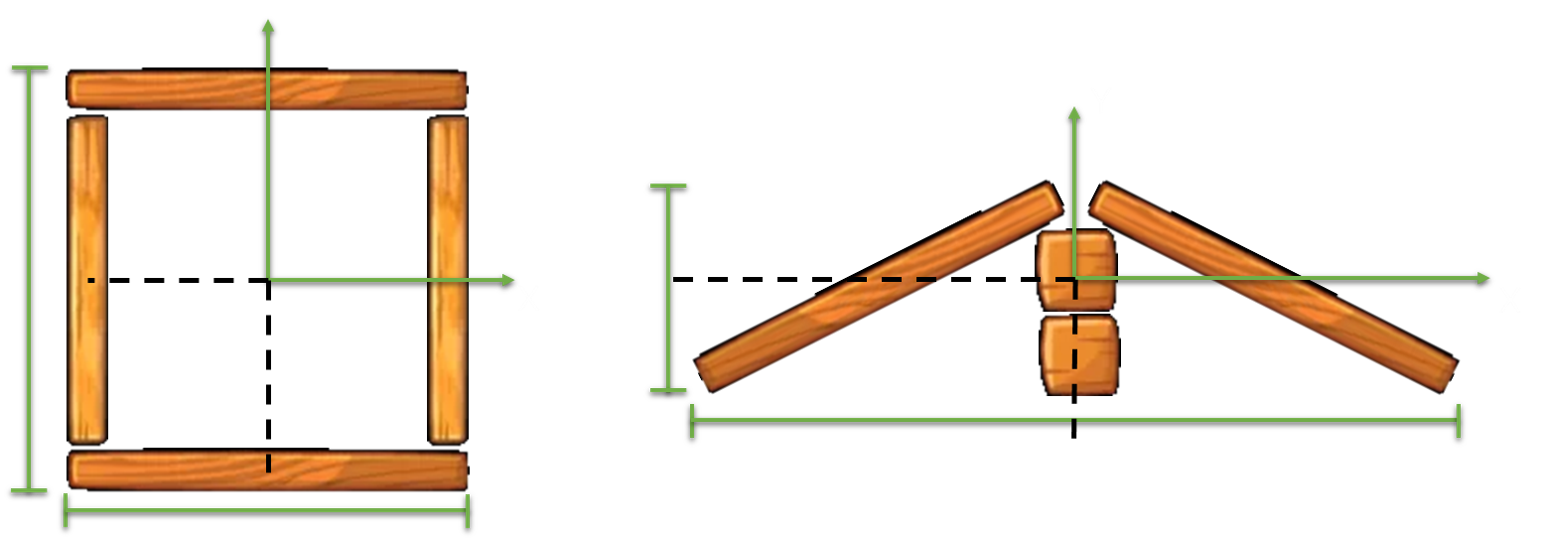
\includegraphics[width=1.0\textwidth]{img/bounding_box_calculation.png}
  \caption{Cálculo de bordes de un conjunto}
  \label{figure:bounding-box-calculation}
\end{figure}

Debido a que los conjuntos son creados antes de la ejecución del algoritmo se
permite que el algoritmo se base únicamente manteniendo los apuntadores a las
composiciones de piezas y solo trabaja con estas mediante las operaciones
genéticas del propio algoritmo, esto permitirá que el algoritmo utilice menos
tiempo identificando posibles composiciones.

Utilizando esta manera de generar los compuestos se utiliza un
algoritmo orientado a objetos, para poder acomodar los elementos y crear los objetos
requeridos según sean necesarios, esto se explica más detalladamente en la
sección \ref{subsection:classorientedidea}.

\subsection{Generación de compuestos mediante objetos de clase}
\label{subsection:classorientedidea}

Para mantener un control de los compuestos, principalmente de las piezas
individuales, se propuso la una jerarquía de clases con
herencia, en donde una clase base contendrá los métodos que las clases derivadas
para obtener valores específicos cuando las piezas requieran,
principalmente estos métodos se encargan de calcular las esquinas de las piezas
particulares las cuales permitirán una vez se tenga un conjunto encontrar la
altura y tamaño total del conjunto, así como el centro del mismo.

Utilizando la estrategia mostrada en la Figura
\ref{figure:bounding-box-calculation} y explicada en el capítulo anterior se
define una clase para los conjuntos de piezas, aquí se utilizan los cálculos de
las clases particulares anteriormente mencionadas para obtener los valores de
bordes y tamaño de los conjuntos, estas clases se crean de acuerdo a los
apuntadores indicados en los individuaos de la población, cuando un apuntador
hace referencia a un grupo se obtienen los datos de las piezas que integran al
conjunto y se crean objetos nuevos de esas mismas clases que pertenecerán a un
individuo particular, esto debido a que al hacer referencia a un objeto
previamente creado un cambio realizado en un individuo particular se propagaría
a todos los individuos que utilicen ese mismo apuntador, por tal motivo cuando
se crean los conjuntos se mantiene una lista de valores que indican la clase que
se deberá de crear y la posición en \textit{x} y \textit{y} relativa al centro
del mismo conjunto.

El sistema de clases se estableció con el fin de reducir la redundancia de
código y para permitir que cada clase particular mantenga los datos necesarios
para crear los objetos que contiene, así como mantener las listas de las piezas
que conforman los niveles antes y después de haber realizado las simulaciones
para poder realizar los cálculos de manera más rápida además de las clases que
controlan los conjuntos y subsecuentemente las piezas individuales. 

\begin{figure}
  \centering
  %%%%%%%%%%%%%%%%%%%%%%%%%%%%%%%%%%%%%%%%%%%%%%%%%%%%%%%%%%%%%%%%
% Class diagram
% Author: Salinas Hernández Jaime
% Version: 1.0 
%%%%%%%%%%%%%%%%%%%%%%%%%%%%%%%%%%%%%%%%%%%%%%%%%%%%%%%%%%%%%%%
\tikzstyle{abstract}=[rectangle, draw=black, rounded corners, fill=blue!40, drop shadow,
        text centered, anchor=north, text=white, text width=4.2cm]
\tikzstyle{comment}=[rectangle, draw=black, rounded corners, fill=green, drop shadow,
        text centered, anchor=north, text=white, text width=4.2cm]
\tikzstyle{myarrow}=[->, >=open triangle 90, thick]
\tikzstyle{line}=[-, thick]
        

\begin{tikzpicture}[node distance=2cm]
    \node (Item) [abstract, rectangle split, align=left, rectangle split parts=3]
        {
            \textbf{Pieza}
            \nodepart{second}string: Material \newline float: X \newline float: Y \newline float: Z \newline
            \nodepart{third}get\_edges \newline as\_dictionary \newline get\_points \newline update\_values
        };
    %\node (ItemInstants) [comment, rectangle split, rectangle split parts=2, below=0.2cm of Item, text justified]
    %    {
    %        \textbf{Methods}
    %        \nodepart{second}
    %            get\_edges
    %            \newline as\_dictionary
    %            \newline get\_points
    %            \newline update\_values
    %    };
    \node (AuxNode01) [text width=4cm, below=3cm of Item] {};
    
    \node (Circle) [abstract, rectangle split, align=left, rectangle split parts=2, left=of AuxNode01]
        {
            \textbf{Circle}
            \nodepart{second}text: "Circle" \newline
            int: Height = 75 \newline
            int: Width = 75
        };
    \node (RectTiny) [abstract, rectangle split, align=left, rectangle split parts=2, right=of Circle]
        {
            \textbf{RectTiny}
            \nodepart{second}text: "RectTiny"\newline int: Height = 25 \newline int: Width = 45
        };
    \node (RectSmall) [abstract, rectangle split, align=left, rectangle split parts=2, right=of RectTiny]
        {
            \textbf{RectSmall}
            \nodepart{second}text: "RectSmall"\newline int: Height = 25 \newline int: Width = 85
        };
    \node (RectMedium) [abstract, rectangle split, align=left, rectangle split parts=2, right=of RectSmall]
        {
            \textbf{RectMedium}
            \nodepart{second}text: "RectMedium"\newline int: Height = 25 \newline int: Width = 165
        };
    \node (RectBig) [abstract, rectangle split, align=left, rectangle split parts=2, right=of RectMedium]
        {
            \textbf{RectBig}
            \nodepart{second}text: "RectBig"\newline int: Height = 25 \newline int: Width = 185
        };
    
    
        
    \node (AuxNode02) [text width=0.5cm, below=of Circle] {};   
    
    \node (RectFat) [abstract, rectangle split, align=left, rectangle split parts=2, left=of AuxNode02]
        {
            \textbf{RectFat}
            \nodepart{second}text: "RectFat"\newline int: Height = 25 \newline int: Width = 85
        };
    \node (SquareTiny) [abstract, rectangle split, align=left, rectangle split parts=2, right=of RectFat]
        {
            \textbf{SquareTiny}
            \nodepart{second}text: "SquareTiny"\newline int: Height = 25 \newline int: Width = 25
        };
    \node (SquareSmall) [abstract, rectangle split, align=left, rectangle split parts=2, right=of SquareTiny]
        {
            \textbf{SquareSmall}
            \nodepart{second}text: "SquareSmall"\newline int: Height = 45 \newline int: Width = 45
        };
    \node (Triangle) [abstract, rectangle split, align=left, rectangle split parts=2, right=of SquareSmall]
        {
            \textbf{Triangle}
            \nodepart{second}text: "Triangle"\newline int: Height = 75 \newline int: Width = 75
        };
    \node (TriangleHole) [abstract, rectangle split, align=left, rectangle split parts=2, right=of Triangle]
        {
            \textbf{TriangleHole}
            \nodepart{second}text: "TriangleHole"\newline int: Height = 85 \newline int: Width = 85
        };
    \node (SquareHole) [abstract, rectangle split, align=left, rectangle split parts=2, right=of TriangleHole]
        {
            \textbf{SquareHole}
            \nodepart{second}text: "SquareHole"\newline int: Height = 85 \newline int: Width = 85
        };
        
    
    
    \draw[myarrow] (RectSmall.north) -- ++(0,0.8) -| (Item.south);
    \draw[line] (Circle.north) -- ++(0,0.8) -| (RectTiny.north);
    \draw[line] (Circle.north) -- ++(0,0.8) -| (RectSmall.north);
    \draw[line] (Circle.north) -- ++(0,0.8) -| (RectMedium.north);
    \draw[line] (Circle.north) -- ++(0,0.8) -| (RectBig.north);
    \draw[line] (Circle.north) -- ++(0,0.8) -| (RectFat.north);
    \draw[line] (Circle.north) -- ++(0,0.8) -| (SquareTiny.east);
    \draw[line] (Circle.north) -- ++(0,0.8) -| (SquareSmall.east);
    \draw[line] (Circle.north) -- ++(0,0.8) -| (Triangle.east);
    \draw[line] (Circle.north) -- ++(0,0.8) -| (TriangleHole.east);
    \draw[line] (Circle.north) -- ++(0,0.8) -| (SquareHole.east);
        
        
\end{tikzpicture}
  \scalebox{.43}{%%%%%%%%%%%%%%%%%%%%%%%%%%%%%%%%%%%%%%%%%%%%%%%%%%%%%%%%%%%%%%%
% Class diagram
% Author: Salinas Hernández Jaime
% Version: 1.0 
%%%%%%%%%%%%%%%%%%%%%%%%%%%%%%%%%%%%%%%%%%%%%%%%%%%%%%%%%%%%%%%
\tikzstyle{abstract}=[rectangle, draw=black, rounded corners, fill=blue!40, drop shadow,
        text centered, anchor=north, text=white, text width=4.2cm]
\tikzstyle{comment}=[rectangle, draw=black, rounded corners, fill=green, drop shadow,
        text centered, anchor=north, text=white, text width=4.2cm]
\tikzstyle{myarrow}=[->, >=open triangle 90, thick]
\tikzstyle{line}=[-, thick]
        

\begin{tikzpicture}[node distance=2cm]
    \node (Item) [abstract, rectangle split, align=left, rectangle split parts=3]
        {
            \textbf{Pieza}
            \nodepart{second}string: Material \newline float: X \newline float: Y \newline float: Z \newline
            \nodepart{third}get\_edges \newline as\_dictionary \newline get\_points \newline update\_values
        };
    %\node (ItemInstants) [comment, rectangle split, rectangle split parts=2, below=0.2cm of Item, text justified]
    %    {
    %        \textbf{Methods}
    %        \nodepart{second}
    %            get\_edges
    %            \newline as\_dictionary
    %            \newline get\_points
    %            \newline update\_values
    %    };
    \node (AuxNode01) [text width=4cm, below=3cm of Item] {};
    
    \node (Circle) [abstract, rectangle split, align=left, rectangle split parts=2, left=of AuxNode01]
        {
            \textbf{Circle}
            \nodepart{second}text: "Circle" \newline
            int: Height = 75 \newline
            int: Width = 75
        };
    \node (RectTiny) [abstract, rectangle split, align=left, rectangle split parts=2, right=of Circle]
        {
            \textbf{RectTiny}
            \nodepart{second}text: "RectTiny"\newline int: Height = 25 \newline int: Width = 45
        };
    \node (RectSmall) [abstract, rectangle split, align=left, rectangle split parts=2, right=of RectTiny]
        {
            \textbf{RectSmall}
            \nodepart{second}text: "RectSmall"\newline int: Height = 25 \newline int: Width = 85
        };
    \node (RectMedium) [abstract, rectangle split, align=left, rectangle split parts=2, right=of RectSmall]
        {
            \textbf{RectMedium}
            \nodepart{second}text: "RectMedium"\newline int: Height = 25 \newline int: Width = 165
        };
    \node (RectBig) [abstract, rectangle split, align=left, rectangle split parts=2, right=of RectMedium]
        {
            \textbf{RectBig}
            \nodepart{second}text: "RectBig"\newline int: Height = 25 \newline int: Width = 185
        };
    
    
        
    \node (AuxNode02) [text width=0.5cm, below=of Circle] {};   
    
    \node (RectFat) [abstract, rectangle split, align=left, rectangle split parts=2, left=of AuxNode02]
        {
            \textbf{RectFat}
            \nodepart{second}text: "RectFat"\newline int: Height = 25 \newline int: Width = 85
        };
    \node (SquareTiny) [abstract, rectangle split, align=left, rectangle split parts=2, right=of RectFat]
        {
            \textbf{SquareTiny}
            \nodepart{second}text: "SquareTiny"\newline int: Height = 25 \newline int: Width = 25
        };
    \node (SquareSmall) [abstract, rectangle split, align=left, rectangle split parts=2, right=of SquareTiny]
        {
            \textbf{SquareSmall}
            \nodepart{second}text: "SquareSmall"\newline int: Height = 45 \newline int: Width = 45
        };
    \node (Triangle) [abstract, rectangle split, align=left, rectangle split parts=2, right=of SquareSmall]
        {
            \textbf{Triangle}
            \nodepart{second}text: "Triangle"\newline int: Height = 75 \newline int: Width = 75
        };
    \node (TriangleHole) [abstract, rectangle split, align=left, rectangle split parts=2, right=of Triangle]
        {
            \textbf{TriangleHole}
            \nodepart{second}text: "TriangleHole"\newline int: Height = 85 \newline int: Width = 85
        };
    \node (SquareHole) [abstract, rectangle split, align=left, rectangle split parts=2, right=of TriangleHole]
        {
            \textbf{SquareHole}
            \nodepart{second}text: "SquareHole"\newline int: Height = 85 \newline int: Width = 85
        };
        
    
    
    \draw[myarrow] (RectSmall.north) -- ++(0,0.8) -| (Item.south);
    \draw[line] (Circle.north) -- ++(0,0.8) -| (RectTiny.north);
    \draw[line] (Circle.north) -- ++(0,0.8) -| (RectSmall.north);
    \draw[line] (Circle.north) -- ++(0,0.8) -| (RectMedium.north);
    \draw[line] (Circle.north) -- ++(0,0.8) -| (RectBig.north);
    \draw[line] (Circle.north) -- ++(0,0.8) -| (RectFat.north);
    \draw[line] (Circle.north) -- ++(0,0.8) -| (SquareTiny.east);
    \draw[line] (Circle.north) -- ++(0,0.8) -| (SquareSmall.east);
    \draw[line] (Circle.north) -- ++(0,0.8) -| (Triangle.east);
    \draw[line] (Circle.north) -- ++(0,0.8) -| (TriangleHole.east);
    \draw[line] (Circle.north) -- ++(0,0.8) -| (SquareHole.east);
        
        
\end{tikzpicture}}
  %\resizebox{.1\linewidth}{!}{%%%%%%%%%%%%%%%%%%%%%%%%%%%%%%%%%%%%%%%%%%%%%%%%%%%%%%%%%%%%%%%
% Class diagram
% Author: Salinas Hernández Jaime
% Version: 1.0 
%%%%%%%%%%%%%%%%%%%%%%%%%%%%%%%%%%%%%%%%%%%%%%%%%%%%%%%%%%%%%%%
\tikzstyle{abstract}=[rectangle, draw=black, rounded corners, fill=blue!40, drop shadow,
        text centered, anchor=north, text=white, text width=4.2cm]
\tikzstyle{comment}=[rectangle, draw=black, rounded corners, fill=green, drop shadow,
        text centered, anchor=north, text=white, text width=4.2cm]
\tikzstyle{myarrow}=[->, >=open triangle 90, thick]
\tikzstyle{line}=[-, thick]
        

\begin{tikzpicture}[node distance=2cm]
    \node (Item) [abstract, rectangle split, align=left, rectangle split parts=3]
        {
            \textbf{Pieza}
            \nodepart{second}string: Material \newline float: X \newline float: Y \newline float: Z \newline
            \nodepart{third}get\_edges \newline as\_dictionary \newline get\_points \newline update\_values
        };
    %\node (ItemInstants) [comment, rectangle split, rectangle split parts=2, below=0.2cm of Item, text justified]
    %    {
    %        \textbf{Methods}
    %        \nodepart{second}
    %            get\_edges
    %            \newline as\_dictionary
    %            \newline get\_points
    %            \newline update\_values
    %    };
    \node (AuxNode01) [text width=4cm, below=3cm of Item] {};
    
    \node (Circle) [abstract, rectangle split, align=left, rectangle split parts=2, left=of AuxNode01]
        {
            \textbf{Circle}
            \nodepart{second}text: "Circle" \newline
            int: Height = 75 \newline
            int: Width = 75
        };
    \node (RectTiny) [abstract, rectangle split, align=left, rectangle split parts=2, right=of Circle]
        {
            \textbf{RectTiny}
            \nodepart{second}text: "RectTiny"\newline int: Height = 25 \newline int: Width = 45
        };
    \node (RectSmall) [abstract, rectangle split, align=left, rectangle split parts=2, right=of RectTiny]
        {
            \textbf{RectSmall}
            \nodepart{second}text: "RectSmall"\newline int: Height = 25 \newline int: Width = 85
        };
    \node (RectMedium) [abstract, rectangle split, align=left, rectangle split parts=2, right=of RectSmall]
        {
            \textbf{RectMedium}
            \nodepart{second}text: "RectMedium"\newline int: Height = 25 \newline int: Width = 165
        };
    \node (RectBig) [abstract, rectangle split, align=left, rectangle split parts=2, right=of RectMedium]
        {
            \textbf{RectBig}
            \nodepart{second}text: "RectBig"\newline int: Height = 25 \newline int: Width = 185
        };
    
    
        
    \node (AuxNode02) [text width=0.5cm, below=of Circle] {};   
    
    \node (RectFat) [abstract, rectangle split, align=left, rectangle split parts=2, left=of AuxNode02]
        {
            \textbf{RectFat}
            \nodepart{second}text: "RectFat"\newline int: Height = 25 \newline int: Width = 85
        };
    \node (SquareTiny) [abstract, rectangle split, align=left, rectangle split parts=2, right=of RectFat]
        {
            \textbf{SquareTiny}
            \nodepart{second}text: "SquareTiny"\newline int: Height = 25 \newline int: Width = 25
        };
    \node (SquareSmall) [abstract, rectangle split, align=left, rectangle split parts=2, right=of SquareTiny]
        {
            \textbf{SquareSmall}
            \nodepart{second}text: "SquareSmall"\newline int: Height = 45 \newline int: Width = 45
        };
    \node (Triangle) [abstract, rectangle split, align=left, rectangle split parts=2, right=of SquareSmall]
        {
            \textbf{Triangle}
            \nodepart{second}text: "Triangle"\newline int: Height = 75 \newline int: Width = 75
        };
    \node (TriangleHole) [abstract, rectangle split, align=left, rectangle split parts=2, right=of Triangle]
        {
            \textbf{TriangleHole}
            \nodepart{second}text: "TriangleHole"\newline int: Height = 85 \newline int: Width = 85
        };
    \node (SquareHole) [abstract, rectangle split, align=left, rectangle split parts=2, right=of TriangleHole]
        {
            \textbf{SquareHole}
            \nodepart{second}text: "SquareHole"\newline int: Height = 85 \newline int: Width = 85
        };
        
    
    
    \draw[myarrow] (RectSmall.north) -- ++(0,0.8) -| (Item.south);
    \draw[line] (Circle.north) -- ++(0,0.8) -| (RectTiny.north);
    \draw[line] (Circle.north) -- ++(0,0.8) -| (RectSmall.north);
    \draw[line] (Circle.north) -- ++(0,0.8) -| (RectMedium.north);
    \draw[line] (Circle.north) -- ++(0,0.8) -| (RectBig.north);
    \draw[line] (Circle.north) -- ++(0,0.8) -| (RectFat.north);
    \draw[line] (Circle.north) -- ++(0,0.8) -| (SquareTiny.east);
    \draw[line] (Circle.north) -- ++(0,0.8) -| (SquareSmall.east);
    \draw[line] (Circle.north) -- ++(0,0.8) -| (Triangle.east);
    \draw[line] (Circle.north) -- ++(0,0.8) -| (TriangleHole.east);
    \draw[line] (Circle.north) -- ++(0,0.8) -| (SquareHole.east);
        
        
\end{tikzpicture}}
  %\includegraphics[width=1.0\textwidth]{img/bounding_box_calculations.png}
  \caption{Diagrama de clase de piezas}
  \label{figure:pieces-class-diagram}
\end{figure}

Estas clases se desarrollaron utilizando herencia y polimorfismo, cómo se
muestra en la Figura \ref{figure:pieces-class-diagram}. Las once clases de las
piezas básicas heredan los métodos de la clase principal, esto es cómo se
menciona anteriormente por que las acciones que las clases particulares harán
serán las mismas sin modificar nada en los métodos, sin embargo, cada una activa
un constructor con los datos de tamaño y nombre específicos, estos datos son
utilizados para las mediciones y para integrar casa pieza particular cómo una
lista de texto que se utilizará para generar los archivos de los niveles.

De igual manera se utiliza una clase específica para controlar la generación de
los conjuntos, la manera en cómo funciona esta clase es que se entrega una lista
al generador de compuestos, esta lista contiene una o más piezas que conformaran
el conjunto particular, la manera en cómo se entregan estas listas es cada línea
de la lista contiene la información necesaria para crear los objetos de clase de
las piezas requeridas, estos elementos se utilizan con las clases previamente
descritas para para generar un conjunto especifico, además de eso esta clase se
encarga de generar las listas y calcular los valores finales de los conjuntos,
siendo estos valores, el punto más alto al centro del conjunto, la altura, el
ancho y las esquinas del mismo, así como un método que permite crear, apoyándose
de las clases particulares obtiene los valores que definen cada elemento del
conjunto, siendo el nombre, material del que esta hecho y los offsets o
distancias desde el centro del conjunto al centro de cada pieza particular.

\begin{figure}
  \centering
  %%%%%%%%%%%%%%%%%%%%%%%%%%%%%%%%%%%%%%%%%%%%%%%%%%%%%%%%%%%%%%%%
% Class diagram
% Author: Salinas Hernández Jaime
% Version: 1.0 
%%%%%%%%%%%%%%%%%%%%%%%%%%%%%%%%%%%%%%%%%%%%%%%%%%%%%%%%%%%%%%%
\tikzstyle{abstract}=[rectangle, draw=black, rounded corners, fill=blue!40, drop shadow,
        text centered, anchor=north, text=white, text width=4.2cm]
\tikzstyle{comment}=[rectangle, draw=black, rounded corners, fill=green, drop shadow,
        text centered, anchor=north, text=white, text width=4.2cm]
\tikzstyle{myarrow}=[->, >=open triangle 90, thick]
\tikzstyle{line}=[-, thick]
        

\begin{tikzpicture}[node distance=2cm]
    \node (Item) [abstract, rectangle split, align=left, rectangle split parts=3]
        {
            \textbf{Pieza}
            \nodepart{second}string: Material \newline float: X \newline float: Y \newline float: Z \newline
            \nodepart{third}get\_edges \newline as\_dictionary \newline get\_points \newline update\_values
        };
    %\node (ItemInstants) [comment, rectangle split, rectangle split parts=2, below=0.2cm of Item, text justified]
    %    {
    %        \textbf{Methods}
    %        \nodepart{second}
    %            get\_edges
    %            \newline as\_dictionary
    %            \newline get\_points
    %            \newline update\_values
    %    };
    \node (AuxNode01) [text width=4cm, below=3cm of Item] {};
    
    \node (Circle) [abstract, rectangle split, align=left, rectangle split parts=2, left=of AuxNode01]
        {
            \textbf{Circle}
            \nodepart{second}text: "Circle" \newline
            int: Height = 75 \newline
            int: Width = 75
        };
    \node (RectTiny) [abstract, rectangle split, align=left, rectangle split parts=2, right=of Circle]
        {
            \textbf{RectTiny}
            \nodepart{second}text: "RectTiny"\newline int: Height = 25 \newline int: Width = 45
        };
    \node (RectSmall) [abstract, rectangle split, align=left, rectangle split parts=2, right=of RectTiny]
        {
            \textbf{RectSmall}
            \nodepart{second}text: "RectSmall"\newline int: Height = 25 \newline int: Width = 85
        };
    \node (RectMedium) [abstract, rectangle split, align=left, rectangle split parts=2, right=of RectSmall]
        {
            \textbf{RectMedium}
            \nodepart{second}text: "RectMedium"\newline int: Height = 25 \newline int: Width = 165
        };
    \node (RectBig) [abstract, rectangle split, align=left, rectangle split parts=2, right=of RectMedium]
        {
            \textbf{RectBig}
            \nodepart{second}text: "RectBig"\newline int: Height = 25 \newline int: Width = 185
        };
    
    
        
    \node (AuxNode02) [text width=0.5cm, below=of Circle] {};   
    
    \node (RectFat) [abstract, rectangle split, align=left, rectangle split parts=2, left=of AuxNode02]
        {
            \textbf{RectFat}
            \nodepart{second}text: "RectFat"\newline int: Height = 25 \newline int: Width = 85
        };
    \node (SquareTiny) [abstract, rectangle split, align=left, rectangle split parts=2, right=of RectFat]
        {
            \textbf{SquareTiny}
            \nodepart{second}text: "SquareTiny"\newline int: Height = 25 \newline int: Width = 25
        };
    \node (SquareSmall) [abstract, rectangle split, align=left, rectangle split parts=2, right=of SquareTiny]
        {
            \textbf{SquareSmall}
            \nodepart{second}text: "SquareSmall"\newline int: Height = 45 \newline int: Width = 45
        };
    \node (Triangle) [abstract, rectangle split, align=left, rectangle split parts=2, right=of SquareSmall]
        {
            \textbf{Triangle}
            \nodepart{second}text: "Triangle"\newline int: Height = 75 \newline int: Width = 75
        };
    \node (TriangleHole) [abstract, rectangle split, align=left, rectangle split parts=2, right=of Triangle]
        {
            \textbf{TriangleHole}
            \nodepart{second}text: "TriangleHole"\newline int: Height = 85 \newline int: Width = 85
        };
    \node (SquareHole) [abstract, rectangle split, align=left, rectangle split parts=2, right=of TriangleHole]
        {
            \textbf{SquareHole}
            \nodepart{second}text: "SquareHole"\newline int: Height = 85 \newline int: Width = 85
        };
        
    
    
    \draw[myarrow] (RectSmall.north) -- ++(0,0.8) -| (Item.south);
    \draw[line] (Circle.north) -- ++(0,0.8) -| (RectTiny.north);
    \draw[line] (Circle.north) -- ++(0,0.8) -| (RectSmall.north);
    \draw[line] (Circle.north) -- ++(0,0.8) -| (RectMedium.north);
    \draw[line] (Circle.north) -- ++(0,0.8) -| (RectBig.north);
    \draw[line] (Circle.north) -- ++(0,0.8) -| (RectFat.north);
    \draw[line] (Circle.north) -- ++(0,0.8) -| (SquareTiny.east);
    \draw[line] (Circle.north) -- ++(0,0.8) -| (SquareSmall.east);
    \draw[line] (Circle.north) -- ++(0,0.8) -| (Triangle.east);
    \draw[line] (Circle.north) -- ++(0,0.8) -| (TriangleHole.east);
    \draw[line] (Circle.north) -- ++(0,0.8) -| (SquareHole.east);
        
        
\end{tikzpicture}
  \scalebox{.65}{%%%%%%%%%%%%%%%%%%%%%%%%%%%%%%%%%%%%%%%%%%%%%%%%%%%%%%%%%%%%%%%
% Class diagram
% Author: Salinas Hernández Jaime
% Version: 1.0 
%%%%%%%%%%%%%%%%%%%%%%%%%%%%%%%%%%%%%%%%%%%%%%%%%%%%%%%%%%%%%%%
\tikzstyle{abstract}=[rectangle, draw=black, rounded corners, fill=blue!40, drop shadow,
        text centered, anchor=north, text=white, text width=4.5cm]
\tikzstyle{comment}=[rectangle, draw=black, rounded corners, fill=green, drop shadow,
        text centered, anchor=north, text=white, text width=4.5cm]
\tikzstyle{myarrow}=[->, >=open triangle 90, thick]
\tikzstyle{line}=[-, thick]
        

\begin{tikzpicture}[node distance=2cm]
    \node (Composite) [abstract, rectangle split, align=left, rectangle split parts=3]
        {
            \textbf{Composite}
            \nodepart{second}float: height \newline 
            float: width \newline 
            list: top\_center \newline 
            list: dictionary \newline
            list: low\_center \newline
            object: Objects \newline
            object: blocks
            \nodepart{third}get\_values \newline 
            get\_top\_center \newline 
            get\_low\_center \newline 
            gen\_dictionary \newline
            move\_xy
        };
        
        
\end{tikzpicture}}
  %\resizebox{.1\linewidth}{!}{%%%%%%%%%%%%%%%%%%%%%%%%%%%%%%%%%%%%%%%%%%%%%%%%%%%%%%%%%%%%%%%
% Class diagram
% Author: Salinas Hernández Jaime
% Version: 1.0 
%%%%%%%%%%%%%%%%%%%%%%%%%%%%%%%%%%%%%%%%%%%%%%%%%%%%%%%%%%%%%%%
\tikzstyle{abstract}=[rectangle, draw=black, rounded corners, fill=blue!40, drop shadow,
        text centered, anchor=north, text=white, text width=4.2cm]
\tikzstyle{comment}=[rectangle, draw=black, rounded corners, fill=green, drop shadow,
        text centered, anchor=north, text=white, text width=4.2cm]
\tikzstyle{myarrow}=[->, >=open triangle 90, thick]
\tikzstyle{line}=[-, thick]
        

\begin{tikzpicture}[node distance=2cm]
    \node (Item) [abstract, rectangle split, align=left, rectangle split parts=3]
        {
            \textbf{Pieza}
            \nodepart{second}string: Material \newline float: X \newline float: Y \newline float: Z \newline
            \nodepart{third}get\_edges \newline as\_dictionary \newline get\_points \newline update\_values
        };
    %\node (ItemInstants) [comment, rectangle split, rectangle split parts=2, below=0.2cm of Item, text justified]
    %    {
    %        \textbf{Methods}
    %        \nodepart{second}
    %            get\_edges
    %            \newline as\_dictionary
    %            \newline get\_points
    %            \newline update\_values
    %    };
    \node (AuxNode01) [text width=4cm, below=3cm of Item] {};
    
    \node (Circle) [abstract, rectangle split, align=left, rectangle split parts=2, left=of AuxNode01]
        {
            \textbf{Circle}
            \nodepart{second}text: "Circle" \newline
            int: Height = 75 \newline
            int: Width = 75
        };
    \node (RectTiny) [abstract, rectangle split, align=left, rectangle split parts=2, right=of Circle]
        {
            \textbf{RectTiny}
            \nodepart{second}text: "RectTiny"\newline int: Height = 25 \newline int: Width = 45
        };
    \node (RectSmall) [abstract, rectangle split, align=left, rectangle split parts=2, right=of RectTiny]
        {
            \textbf{RectSmall}
            \nodepart{second}text: "RectSmall"\newline int: Height = 25 \newline int: Width = 85
        };
    \node (RectMedium) [abstract, rectangle split, align=left, rectangle split parts=2, right=of RectSmall]
        {
            \textbf{RectMedium}
            \nodepart{second}text: "RectMedium"\newline int: Height = 25 \newline int: Width = 165
        };
    \node (RectBig) [abstract, rectangle split, align=left, rectangle split parts=2, right=of RectMedium]
        {
            \textbf{RectBig}
            \nodepart{second}text: "RectBig"\newline int: Height = 25 \newline int: Width = 185
        };
    
    
        
    \node (AuxNode02) [text width=0.5cm, below=of Circle] {};   
    
    \node (RectFat) [abstract, rectangle split, align=left, rectangle split parts=2, left=of AuxNode02]
        {
            \textbf{RectFat}
            \nodepart{second}text: "RectFat"\newline int: Height = 25 \newline int: Width = 85
        };
    \node (SquareTiny) [abstract, rectangle split, align=left, rectangle split parts=2, right=of RectFat]
        {
            \textbf{SquareTiny}
            \nodepart{second}text: "SquareTiny"\newline int: Height = 25 \newline int: Width = 25
        };
    \node (SquareSmall) [abstract, rectangle split, align=left, rectangle split parts=2, right=of SquareTiny]
        {
            \textbf{SquareSmall}
            \nodepart{second}text: "SquareSmall"\newline int: Height = 45 \newline int: Width = 45
        };
    \node (Triangle) [abstract, rectangle split, align=left, rectangle split parts=2, right=of SquareSmall]
        {
            \textbf{Triangle}
            \nodepart{second}text: "Triangle"\newline int: Height = 75 \newline int: Width = 75
        };
    \node (TriangleHole) [abstract, rectangle split, align=left, rectangle split parts=2, right=of Triangle]
        {
            \textbf{TriangleHole}
            \nodepart{second}text: "TriangleHole"\newline int: Height = 85 \newline int: Width = 85
        };
    \node (SquareHole) [abstract, rectangle split, align=left, rectangle split parts=2, right=of TriangleHole]
        {
            \textbf{SquareHole}
            \nodepart{second}text: "SquareHole"\newline int: Height = 85 \newline int: Width = 85
        };
        
    
    
    \draw[myarrow] (RectSmall.north) -- ++(0,0.8) -| (Item.south);
    \draw[line] (Circle.north) -- ++(0,0.8) -| (RectTiny.north);
    \draw[line] (Circle.north) -- ++(0,0.8) -| (RectSmall.north);
    \draw[line] (Circle.north) -- ++(0,0.8) -| (RectMedium.north);
    \draw[line] (Circle.north) -- ++(0,0.8) -| (RectBig.north);
    \draw[line] (Circle.north) -- ++(0,0.8) -| (RectFat.north);
    \draw[line] (Circle.north) -- ++(0,0.8) -| (SquareTiny.east);
    \draw[line] (Circle.north) -- ++(0,0.8) -| (SquareSmall.east);
    \draw[line] (Circle.north) -- ++(0,0.8) -| (Triangle.east);
    \draw[line] (Circle.north) -- ++(0,0.8) -| (TriangleHole.east);
    \draw[line] (Circle.north) -- ++(0,0.8) -| (SquareHole.east);
        
        
\end{tikzpicture}}
  %\includegraphics[width=1.0\textwidth]{img/bounding_box_calculations.png}
  \caption{Diagrama de clase de Composite}
  \label{figure:composite-class-diagram}
\end{figure}

Finalmente, debido a que se requiere controlar una gran cantidad de datos
necesarios para el algoritmo genético por cada individuo se utiliza también una
clase extra para ellos, esta clase permite que cada individuo mantenga los
resultados de fitness después de las simulaciones, así como también controlar el
número y listado de las piezas que conformaran cada nivel que representa el
individuo, además de esto la clase permite que los individuos generen los
archivos necesarios de los niveles para ser evaluados, el modelo básico de esta
clase se muestra en la Figura \ref{figure:composite-class-diagram} en donde se
puede ver los elementos que utiliza la clase cómo variables principales así cómo
los métodos que es capaz de ejecutar una vez iniciado el algoritmo.

\begin{figure}
  \centering
  %%%%%%%%%%%%%%%%%%%%%%%%%%%%%%%%%%%%%%%%%%%%%%%%%%%%%%%%%%%%%%%%
% Class diagram
% Author: Salinas Hernández Jaime
% Version: 1.0 
%%%%%%%%%%%%%%%%%%%%%%%%%%%%%%%%%%%%%%%%%%%%%%%%%%%%%%%%%%%%%%%
\tikzstyle{abstract}=[rectangle, draw=black, rounded corners, fill=blue!40, drop shadow,
        text centered, anchor=north, text=white, text width=4.2cm]
\tikzstyle{comment}=[rectangle, draw=black, rounded corners, fill=green, drop shadow,
        text centered, anchor=north, text=white, text width=4.2cm]
\tikzstyle{myarrow}=[->, >=open triangle 90, thick]
\tikzstyle{line}=[-, thick]
        

\begin{tikzpicture}[node distance=2cm]
    \node (Item) [abstract, rectangle split, align=left, rectangle split parts=3]
        {
            \textbf{Pieza}
            \nodepart{second}string: Material \newline float: X \newline float: Y \newline float: Z \newline
            \nodepart{third}get\_edges \newline as\_dictionary \newline get\_points \newline update\_values
        };
    %\node (ItemInstants) [comment, rectangle split, rectangle split parts=2, below=0.2cm of Item, text justified]
    %    {
    %        \textbf{Methods}
    %        \nodepart{second}
    %            get\_edges
    %            \newline as\_dictionary
    %            \newline get\_points
    %            \newline update\_values
    %    };
    \node (AuxNode01) [text width=4cm, below=3cm of Item] {};
    
    \node (Circle) [abstract, rectangle split, align=left, rectangle split parts=2, left=of AuxNode01]
        {
            \textbf{Circle}
            \nodepart{second}text: "Circle" \newline
            int: Height = 75 \newline
            int: Width = 75
        };
    \node (RectTiny) [abstract, rectangle split, align=left, rectangle split parts=2, right=of Circle]
        {
            \textbf{RectTiny}
            \nodepart{second}text: "RectTiny"\newline int: Height = 25 \newline int: Width = 45
        };
    \node (RectSmall) [abstract, rectangle split, align=left, rectangle split parts=2, right=of RectTiny]
        {
            \textbf{RectSmall}
            \nodepart{second}text: "RectSmall"\newline int: Height = 25 \newline int: Width = 85
        };
    \node (RectMedium) [abstract, rectangle split, align=left, rectangle split parts=2, right=of RectSmall]
        {
            \textbf{RectMedium}
            \nodepart{second}text: "RectMedium"\newline int: Height = 25 \newline int: Width = 165
        };
    \node (RectBig) [abstract, rectangle split, align=left, rectangle split parts=2, right=of RectMedium]
        {
            \textbf{RectBig}
            \nodepart{second}text: "RectBig"\newline int: Height = 25 \newline int: Width = 185
        };
    
    
        
    \node (AuxNode02) [text width=0.5cm, below=of Circle] {};   
    
    \node (RectFat) [abstract, rectangle split, align=left, rectangle split parts=2, left=of AuxNode02]
        {
            \textbf{RectFat}
            \nodepart{second}text: "RectFat"\newline int: Height = 25 \newline int: Width = 85
        };
    \node (SquareTiny) [abstract, rectangle split, align=left, rectangle split parts=2, right=of RectFat]
        {
            \textbf{SquareTiny}
            \nodepart{second}text: "SquareTiny"\newline int: Height = 25 \newline int: Width = 25
        };
    \node (SquareSmall) [abstract, rectangle split, align=left, rectangle split parts=2, right=of SquareTiny]
        {
            \textbf{SquareSmall}
            \nodepart{second}text: "SquareSmall"\newline int: Height = 45 \newline int: Width = 45
        };
    \node (Triangle) [abstract, rectangle split, align=left, rectangle split parts=2, right=of SquareSmall]
        {
            \textbf{Triangle}
            \nodepart{second}text: "Triangle"\newline int: Height = 75 \newline int: Width = 75
        };
    \node (TriangleHole) [abstract, rectangle split, align=left, rectangle split parts=2, right=of Triangle]
        {
            \textbf{TriangleHole}
            \nodepart{second}text: "TriangleHole"\newline int: Height = 85 \newline int: Width = 85
        };
    \node (SquareHole) [abstract, rectangle split, align=left, rectangle split parts=2, right=of TriangleHole]
        {
            \textbf{SquareHole}
            \nodepart{second}text: "SquareHole"\newline int: Height = 85 \newline int: Width = 85
        };
        
    
    
    \draw[myarrow] (RectSmall.north) -- ++(0,0.8) -| (Item.south);
    \draw[line] (Circle.north) -- ++(0,0.8) -| (RectTiny.north);
    \draw[line] (Circle.north) -- ++(0,0.8) -| (RectSmall.north);
    \draw[line] (Circle.north) -- ++(0,0.8) -| (RectMedium.north);
    \draw[line] (Circle.north) -- ++(0,0.8) -| (RectBig.north);
    \draw[line] (Circle.north) -- ++(0,0.8) -| (RectFat.north);
    \draw[line] (Circle.north) -- ++(0,0.8) -| (SquareTiny.east);
    \draw[line] (Circle.north) -- ++(0,0.8) -| (SquareSmall.east);
    \draw[line] (Circle.north) -- ++(0,0.8) -| (Triangle.east);
    \draw[line] (Circle.north) -- ++(0,0.8) -| (TriangleHole.east);
    \draw[line] (Circle.north) -- ++(0,0.8) -| (SquareHole.east);
        
        
\end{tikzpicture}
  \scalebox{.65}{%%%%%%%%%%%%%%%%%%%%%%%%%%%%%%%%%%%%%%%%%%%%%%%%%%%%%%%%%%%%%%%
% Class diagram
% Author: Salinas Hernández Jaime
% Version: 1.0 
%%%%%%%%%%%%%%%%%%%%%%%%%%%%%%%%%%%%%%%%%%%%%%%%%%%%%%%%%%%%%%%
\tikzstyle{abstract}=[rectangle, draw=black, rounded corners, fill=blue!40, drop shadow,
        text centered, anchor=north, text=white, text width=5cm]
\tikzstyle{comment}=[rectangle, draw=black, rounded corners, fill=green, drop shadow,
        text centered, anchor=north, text=white, text width=5cm]
\tikzstyle{myarrow}=[->, >=open triangle 90, thick]
\tikzstyle{line}=[-, thick]
        

\begin{tikzpicture}[node distance=2cm]
    \node (Individual) [abstract, rectangle split, align=left, rectangle split parts=3]
        {
            \textbf{Individual}
            \nodepart{second}list: chromosome \newline 
            list: mask \newline 
            list: chromosome\_objects\newline 
            list: object\_list
            \nodepart{third}update\_mutation \newline 
            object\_list\_gen \newline 
            generate\_xml \newline 
            read\_xml \newline
            read\_xml\_tourney \newline
            assign\_mask \newline
            combine\_mask \newline
            get\_fitness \newline
            generate\_xml\_masked \newline
            generate\_xml\_tournery \newline
            generate\_xml\_elite
        };
        
        
\end{tikzpicture}}
  %\resizebox{.1\linewidth}{!}{%%%%%%%%%%%%%%%%%%%%%%%%%%%%%%%%%%%%%%%%%%%%%%%%%%%%%%%%%%%%%%%
% Class diagram
% Author: Salinas Hernández Jaime
% Version: 1.0 
%%%%%%%%%%%%%%%%%%%%%%%%%%%%%%%%%%%%%%%%%%%%%%%%%%%%%%%%%%%%%%%
\tikzstyle{abstract}=[rectangle, draw=black, rounded corners, fill=blue!40, drop shadow,
        text centered, anchor=north, text=white, text width=4.2cm]
\tikzstyle{comment}=[rectangle, draw=black, rounded corners, fill=green, drop shadow,
        text centered, anchor=north, text=white, text width=4.2cm]
\tikzstyle{myarrow}=[->, >=open triangle 90, thick]
\tikzstyle{line}=[-, thick]
        

\begin{tikzpicture}[node distance=2cm]
    \node (Item) [abstract, rectangle split, align=left, rectangle split parts=3]
        {
            \textbf{Pieza}
            \nodepart{second}string: Material \newline float: X \newline float: Y \newline float: Z \newline
            \nodepart{third}get\_edges \newline as\_dictionary \newline get\_points \newline update\_values
        };
    %\node (ItemInstants) [comment, rectangle split, rectangle split parts=2, below=0.2cm of Item, text justified]
    %    {
    %        \textbf{Methods}
    %        \nodepart{second}
    %            get\_edges
    %            \newline as\_dictionary
    %            \newline get\_points
    %            \newline update\_values
    %    };
    \node (AuxNode01) [text width=4cm, below=3cm of Item] {};
    
    \node (Circle) [abstract, rectangle split, align=left, rectangle split parts=2, left=of AuxNode01]
        {
            \textbf{Circle}
            \nodepart{second}text: "Circle" \newline
            int: Height = 75 \newline
            int: Width = 75
        };
    \node (RectTiny) [abstract, rectangle split, align=left, rectangle split parts=2, right=of Circle]
        {
            \textbf{RectTiny}
            \nodepart{second}text: "RectTiny"\newline int: Height = 25 \newline int: Width = 45
        };
    \node (RectSmall) [abstract, rectangle split, align=left, rectangle split parts=2, right=of RectTiny]
        {
            \textbf{RectSmall}
            \nodepart{second}text: "RectSmall"\newline int: Height = 25 \newline int: Width = 85
        };
    \node (RectMedium) [abstract, rectangle split, align=left, rectangle split parts=2, right=of RectSmall]
        {
            \textbf{RectMedium}
            \nodepart{second}text: "RectMedium"\newline int: Height = 25 \newline int: Width = 165
        };
    \node (RectBig) [abstract, rectangle split, align=left, rectangle split parts=2, right=of RectMedium]
        {
            \textbf{RectBig}
            \nodepart{second}text: "RectBig"\newline int: Height = 25 \newline int: Width = 185
        };
    
    
        
    \node (AuxNode02) [text width=0.5cm, below=of Circle] {};   
    
    \node (RectFat) [abstract, rectangle split, align=left, rectangle split parts=2, left=of AuxNode02]
        {
            \textbf{RectFat}
            \nodepart{second}text: "RectFat"\newline int: Height = 25 \newline int: Width = 85
        };
    \node (SquareTiny) [abstract, rectangle split, align=left, rectangle split parts=2, right=of RectFat]
        {
            \textbf{SquareTiny}
            \nodepart{second}text: "SquareTiny"\newline int: Height = 25 \newline int: Width = 25
        };
    \node (SquareSmall) [abstract, rectangle split, align=left, rectangle split parts=2, right=of SquareTiny]
        {
            \textbf{SquareSmall}
            \nodepart{second}text: "SquareSmall"\newline int: Height = 45 \newline int: Width = 45
        };
    \node (Triangle) [abstract, rectangle split, align=left, rectangle split parts=2, right=of SquareSmall]
        {
            \textbf{Triangle}
            \nodepart{second}text: "Triangle"\newline int: Height = 75 \newline int: Width = 75
        };
    \node (TriangleHole) [abstract, rectangle split, align=left, rectangle split parts=2, right=of Triangle]
        {
            \textbf{TriangleHole}
            \nodepart{second}text: "TriangleHole"\newline int: Height = 85 \newline int: Width = 85
        };
    \node (SquareHole) [abstract, rectangle split, align=left, rectangle split parts=2, right=of TriangleHole]
        {
            \textbf{SquareHole}
            \nodepart{second}text: "SquareHole"\newline int: Height = 85 \newline int: Width = 85
        };
        
    
    
    \draw[myarrow] (RectSmall.north) -- ++(0,0.8) -| (Item.south);
    \draw[line] (Circle.north) -- ++(0,0.8) -| (RectTiny.north);
    \draw[line] (Circle.north) -- ++(0,0.8) -| (RectSmall.north);
    \draw[line] (Circle.north) -- ++(0,0.8) -| (RectMedium.north);
    \draw[line] (Circle.north) -- ++(0,0.8) -| (RectBig.north);
    \draw[line] (Circle.north) -- ++(0,0.8) -| (RectFat.north);
    \draw[line] (Circle.north) -- ++(0,0.8) -| (SquareTiny.east);
    \draw[line] (Circle.north) -- ++(0,0.8) -| (SquareSmall.east);
    \draw[line] (Circle.north) -- ++(0,0.8) -| (Triangle.east);
    \draw[line] (Circle.north) -- ++(0,0.8) -| (TriangleHole.east);
    \draw[line] (Circle.north) -- ++(0,0.8) -| (SquareHole.east);
        
        
\end{tikzpicture}}
  %\includegraphics[width=1.0\textwidth]{img/bounding_box_calculations.png}
  \caption{Diagrama de clase de Individuo}
  \label{figure:individual-class-diagram}
\end{figure}

Mediante el uso de estas clases se controla la generación de individuos de tal
manera que un cambio realizado en la clase principal de un individuo deberá de
propagarse hasta la base del mismo siendo estos el controlador de conjuntos y
las piezas individuales, de esta manera las modificaciones realizadas por las
operaciones genéticas de igual manera se deberán de propagar por todo el
individuo realizando las actualizaciones y modificaciones necesarias en las
posiciones y tipos de piezas utilizadas. Cómo se ha mencionado a lo largo de
esta sección el uso de clases para controlar los aspectos básicos de los
individuos resultó de gran utilidad, una de las maneras anteriores de controlar
este aspecto fue mediante el uso individual de métodos para realizar las
modificaciones de los individuos de manera más detallada sin embargo el sistema
de clases permitía que muchos de los métodos se fusionaran de tal manera que
todos los individuos, compuestos y piezas particulares cuentan con los métodos
que utilizarán desde el inicio en lugar de estar llamando los mismos mandando la
información de cada individuo de manera particular, sino que al estar integrados
en los individuos es posible simplemente llamar los parámetros de clase según
sean requeridos, la manera que se tenía anteriormente de utilizar métodos
particulares para la generación, modificación y evolución de los individuos se
explica más adelante en la sección \ref{section:previous-proposed-methods} junto
con otras ideas que no fueron utilizadas o fueron modificadas.

\subsection{Generar niveles utilizando algoritmos genéticos}
\label{subsection:generate-levels-using-GA}

Utilizando las ideas anteriormente presentadas, se llegó a la definición del
algoritmo genético, se decidó que deberá de ser lo que se utilizaría para
representar a los individuos de la población dentro del algoritmo, así como el
que sería lo que evolucionaría y evaluaría, mientras que el sistema de clases
permite tener un control de que es lo que englobará a un individuo el algoritmo
genético es el que a final de cuentas se encargará de realizar la evolución
necesaria mediante los parámetros propuestos, para esto primero se decidió que
sería lo que se alimentaria en el algoritmo para realizar la evaluación de los
individuos, para este valor o variable se decidió que lo que se alimentaria
sería el listado de posiciones de piezas en el individuo, esto es primero se
ejecutaría una instancia del juego con los individuos existentes al momento y se
evaluaría la posición final de las piezas contra la misma posición de las piezas
antes de entrar a la simulación de esta manera lo el valor de fitness de los
individuos sería el total de piezas restantes en el nivel, así como el que tan
bien logran conservar sus posiciones originales dentro de la simulación, esto es
debido a que se busca crear niveles que logren conservar su forma sin ser
manipuladas por el jugador, de igual manera se decidió que sería lo que se
utilizaría para evolucionar a los individuos, en este aspecto se decidió
utilizar una lista de valores enteros que representan a los individuos, esta
lista se explica más a detalle en la sección \ref{chapter:implementation} esta
lista se utilizará dentro del algoritmo genético para realizar las operaciones
genéticas necesarias para crear a los nuevos individuos de la población. 

El diagrama del sistema se muestra en la Figura \ref{figure:algorithm_model}, en
este diagrama se muestra el proceso por el cual pasa el algoritmo genético, desde
el inicio que utiliza un archivo con los parámetros de configuración necesarios
para inicializar el sistema, así como el proceso por el cual pasan los
individuos para su evaluación, de igual manera los individuos pasan por un
proceso de selección en el cual los mejores o en este caso el mejoro individuo
es seleccionado para entrar a un grupo especial con el fin de ser integrado de
vuelta a la población en generaciones subsecuentes para encaminar al algoritmo a
obtener el mejor valor de fitness posible, de igual manera este proceso se
explica más a detalle en el capítulo siguiente en donde se muestra cómo los
conceptos vistos en este capítulo fueron implementados para generación del
sistema.

\begin{figure}
  \centering
  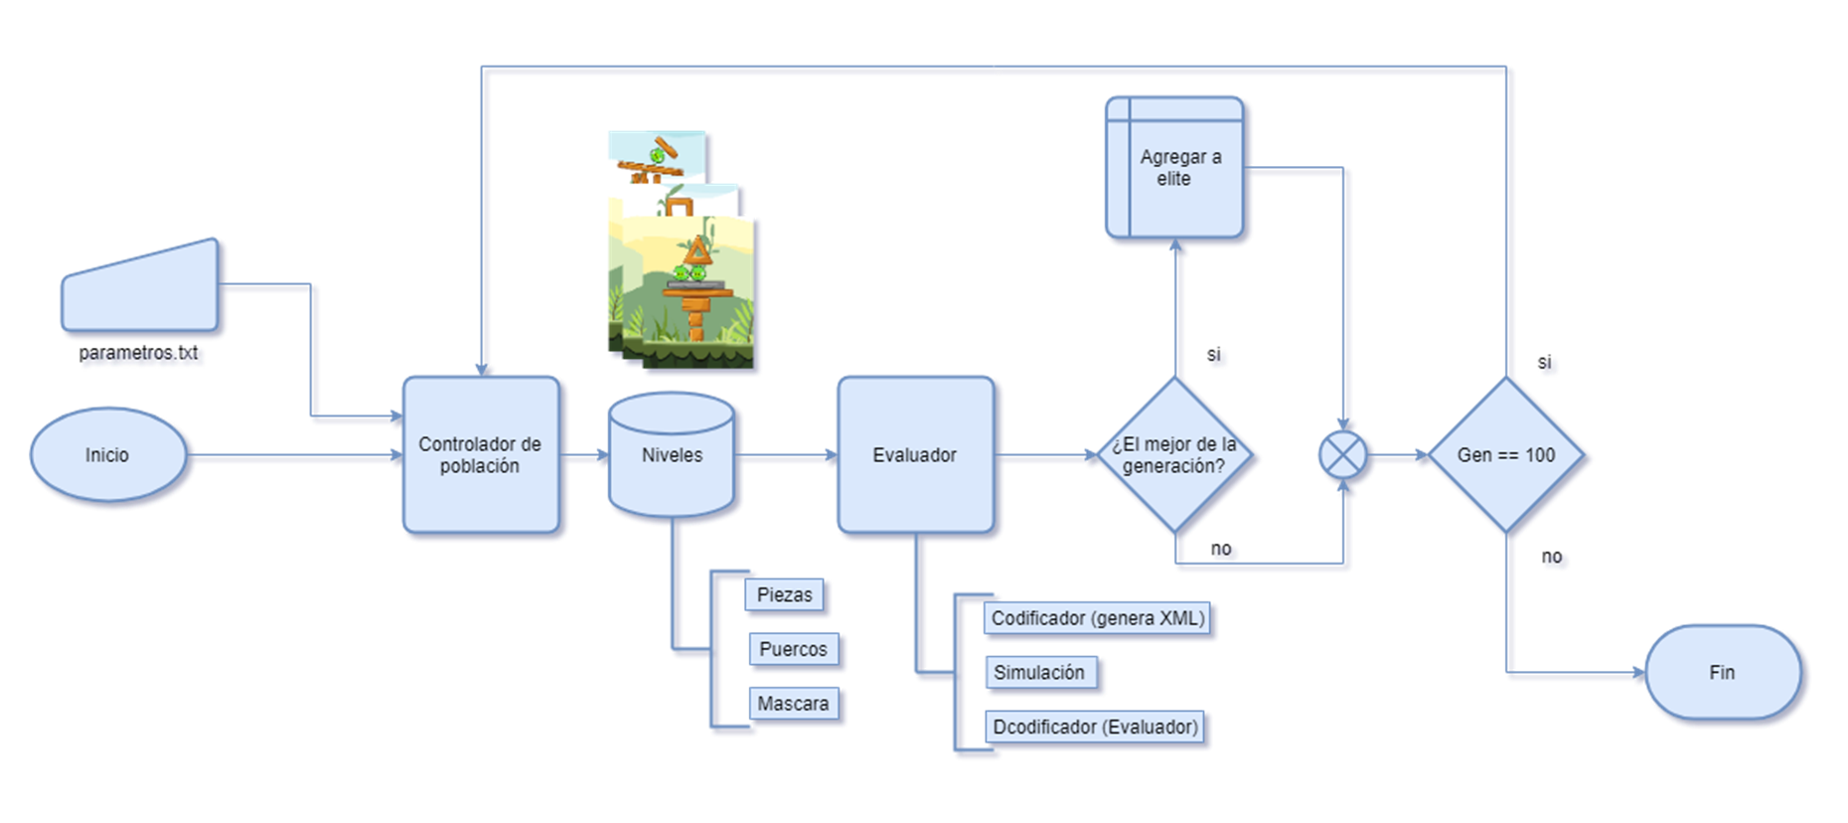
\includegraphics[width=1.0\textwidth]{img/system_model.png}
  \caption{Diagrama de flujo del algoritmo}
  \label{figure:algorithm_model}
\end{figure}

\section{Propuestas anteriores}
\label{section:previous-proposed-methods}

Dentro del aspecto de generar compuestos nuevos para ser utilizados, previamente
se propuso utilizar los resultados de un nivel cómo compuestos para las
siguientes generaciones, un ejemplo de esto se muestra en la Figura
\ref{figure:prev_composite_proposal_bef_aft} en donde una estructura generada
mediante el algoritmo genético se simula en el juego y después de varios
segundos el resultante del mismo podía ser utilizado cómo un compuesto para la
siguiente generación, este método proveería una manera de tener compuestos
verificados cómo viables, sin embargo, se optó por utilizar el generador de
compuestos antes de entrar al ciclo del algoritmo genético.

\begin{figure}
  \centering
  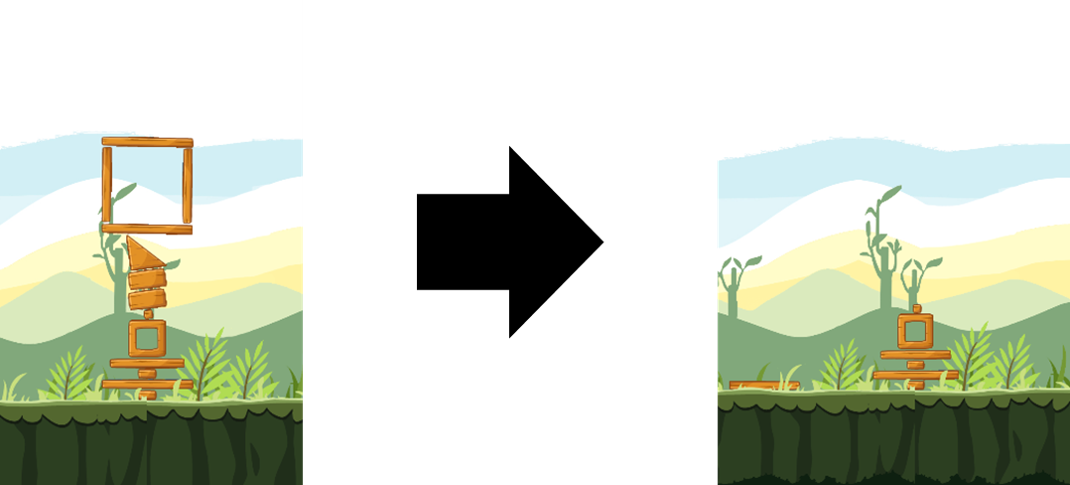
\includegraphics[width=1.0\textwidth]{img/simulation_bef_aft_example.png}
  \caption{Ejemplo de una estructura antes(izquierda) y después(derecha) de una simulación}
  \label{figure:prev_composite_proposal_bef_aft}
\end{figure}

\subsection{Propuesta orientada a métodos}
\label{subsection:objectorientedidea}

Una de las maneras en las que se propuso originalmente el desarrollo del proyecto
fue mediante el uso de diccionarios en Python, esto permitiría
tener un control de los compuestos generados debido a que mediante el uso de
diccionarios se podía generar un apuntados que permitiría que al momento de
generar los cromosomas de los individuos de la población estos utilizarán
simplemente listas numéricas que hicieran referencia al compuesto al cual
pertenecían, esto al final permitiría generar un solo diccionario que
contuviera todos los apuntadores a los compuestos generados.

Esto sin embargo presentó un problema para la generación de nuevos compuestos
debido a que en caso de querer realizar pruebas restringiendo el uso de ciertas
piezas o ciertas combinaciones de material-pieza se tenía que cambiar cada
elemento en el diccionario generado, además de esto se requería que las
piezas pudieran no solo restringirse, sino que se pudieran realizar cambios en
las maneras de cómo se generaban de manera sencilla, por tal se descartó esta
propuesta con el fin de utilizar la propuesta de generación de elementos
mediante el uso de clases cómo se explicó en el capítulo
\ref{subsection:classorientedidea}.

Además de esto otro de los problemas que se presentaban mediante el uso de
métodos para la generación de los cromosomas fue que los métodos se asignaban de
manera directa a los individuos lo cual provocaba que simplemente se asignaran
diccionarios que especifican el conjunto de métodos que se deberían de llamar,
sin embargo, al no tener los beneficios de un sistema de clases que puede ser
re-instanciado en caso de ser requerido se tiene el problema de que cada que se
realiza una modificación en los métodos, los cambios se propagan a los
demás individuos provocando errores en los niveles generados.


\subsection{Regla de tercios}
\label{subsection:ruleofthirds}

Uno de los temas que más interesaba en la generación de niveles fue la manera en
cómo se acomodarían las estructuras en al área del juego, debido a que lo que se
buscó en el proyecto originalmente fue crear estructuras que tuvieran una gran
altura y lograran mantenerse estables se buscaron maneras de lograr que el
posicionamiento de las piezas o compuestos fuese lo más \textit{'controlado'}
posible debido a que simplemente colocar piezas al azar generaría demasiada incongruencia
en los niveles generados, por tal motivo una de las primeras propuestas fue el
uso de la \textit{regla de tercios}.

La regla de tercios es una técnica utilizada en el área de fotografía cuyo
propósito es crear imágenes estéticamente agradables a la vista en donde el
punto focal o punto de interés se encuentra colocado en la alguna de las áreas
de la imagen, un ejemplo de esto se puede apreciar en la Figura
\ref{figure:ruleofthirdsexample} en donde el objeto principal que se quiere
resaltar se trata de colocar en el área central de la imagen completa.

La regla de tercios hace uso de líneas imaginarias que dividen la imagen en nueve
áreas, y mediante el uso de la
cuadricula generada se colocan los objetos principales de una imagen entre
líneas divisorias de tal manera que en caso de imágenes grandes donde existen dos
o más elementos importantes un solo objeto no tome el centro absoluto de la
imagen, sino que se mantenga alineado a un punto donde las líneas se cruzan para
que los demás elementos de la imagen tengan un mismo nivel de interés y en el
caso de que solo sea un elemento no utilice toda la parte central de la imagen
sino que exista un nivel de balance en la imagen en donde el cielo o el fondo
tenga una tercera parte del espacio de la fotografía, mientras que el área
activa o el área inmediatamente adyacente al sujeto de la imagen cubra el
resto de la misma.

La manera en cómo se planeó utilizar esta técnica es mediante el uso de una
cuadricula de tres por tres de la misma manera que se me muestra en la Figura
\ref{figure:ruleofthirdsexample}, pero en el caso de los niveles generados se
espera utilizar la cuadricula para rellenar áreas del nivel iniciando desde la
parte inferior para generar niveles más robustos en sentido de que la
distribución de las piezas es más enfocada al centro creando una pirámide o
llenando todas las áreas dependiendo de la cantidad de piezas utilizadas. 

\begin{figure}
  \centering
  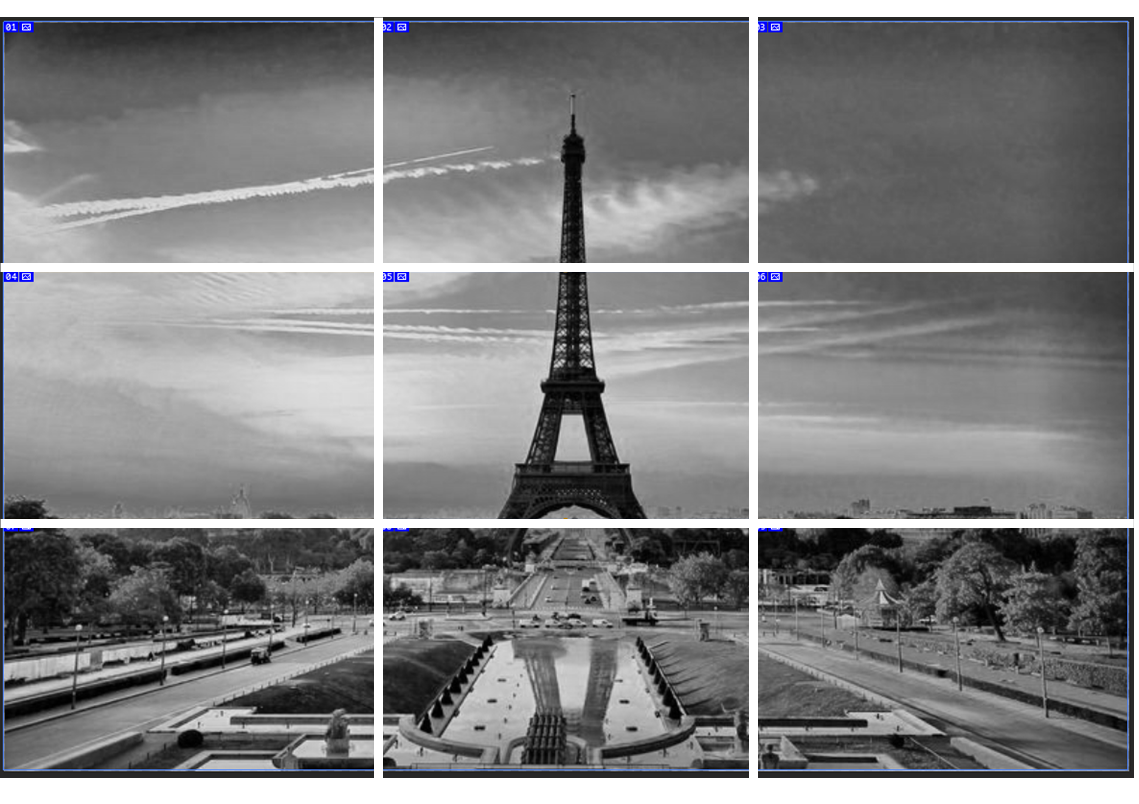
\includegraphics[width=1.0\textwidth]{img/ruleofthirds_example.png}
  \caption{Ejemplo del uso de la regla de tercios en una imagen, el punto de interés se encuentra en la parte central}
  \label{figure:ruleofthirdsexample}
\end{figure}

Debido a que los niveles generados tienen un área de visión o área jugable
variante hasta cierto punto, se definirá un área de juego estática para los
niveles de tal forma que todos siempre se generen con las mismas dimensiones, de
esta manera se evita el tener que estar calculando áreas para los nueve
cuadrantes utilizando la regla de tercios y se utilizan siempre los mismos
valores para distribuir las piezas en los niveles.

El uso de la regla de tercios dentro
del proyecto fue mediante la utilización de máscaras de generación, estas máscaras se
generaron mediante la modificación de la idea detrás de la regla de tercios,
esto se utilizó de igual manera una cuadricula que cubriera el área de juego, la
cuadricula se modificó para cubriera el área con un tamaño de 3 cuadros de
altura y 7 cuadros de largo, de esta manera las piezas tendrían un poco más de
libertad sobre el dónde sería posible colocarlas, el ejemplo básico de la idea
detrás del uso de la regla de tercios se muestra en la Figura
\ref{figure:ruleofthird_on_pieces} en donde se utiliza una máscara simple para
acomodar los elementos en un individuo de tal manera que el ordenamiento dentro
de la cuadricula permitiría la generación de estructuras más complejas, sin
embargo esta idea a pesar de proveer una buena mecánica en el acomodo de las
piezas conllevaba un error debido que no solo se debería de buscar los puntos en
los cuales los elementos se podrían apoyar entre ellos, si no que era requerido
tomar en cuenta las posiciones, alturas, tamaños y ángulos de todos los
elementos presentes en el cromosoma una vez colocados en el nivel, los
resultados obtenidos utilizando la regla de tercios se muestran en la Figura
\ref{figure:ruleofthird_on_chromosome}, en esta imagen se muestra cómo una
máscara pre-generada con una forma de castillo mostrada del lado izquierdo de la
imagen se combina con el cromosoma entrante de un individuo para generar el
nivel mostrado del lado derecho de la imagen, este nivel se trata de asemejar a
lo establecido en la máscara, mientras que el uso de máscaras pre-generadas
permite encaminar el sistema de generación a un conjunto de resultados de igual
manera inhibe que se logre tener una diversidad de niveles debido a que siempre
se mantendrán dentro de las formas especificadas por las máscaras, debido a esto
se optó por modificar la idea para permitir que los individuos tengan una
máscara no pre-generada, sino que de manera pseudoaleatoria se les asigna una
máscara que contendrá de igual manera varias columnas en donde el total de
piezas se reparte de manera aleatoria, esto permitirá tener más diversidad en
los niveles generados.

\begin{figure}
  \centering
  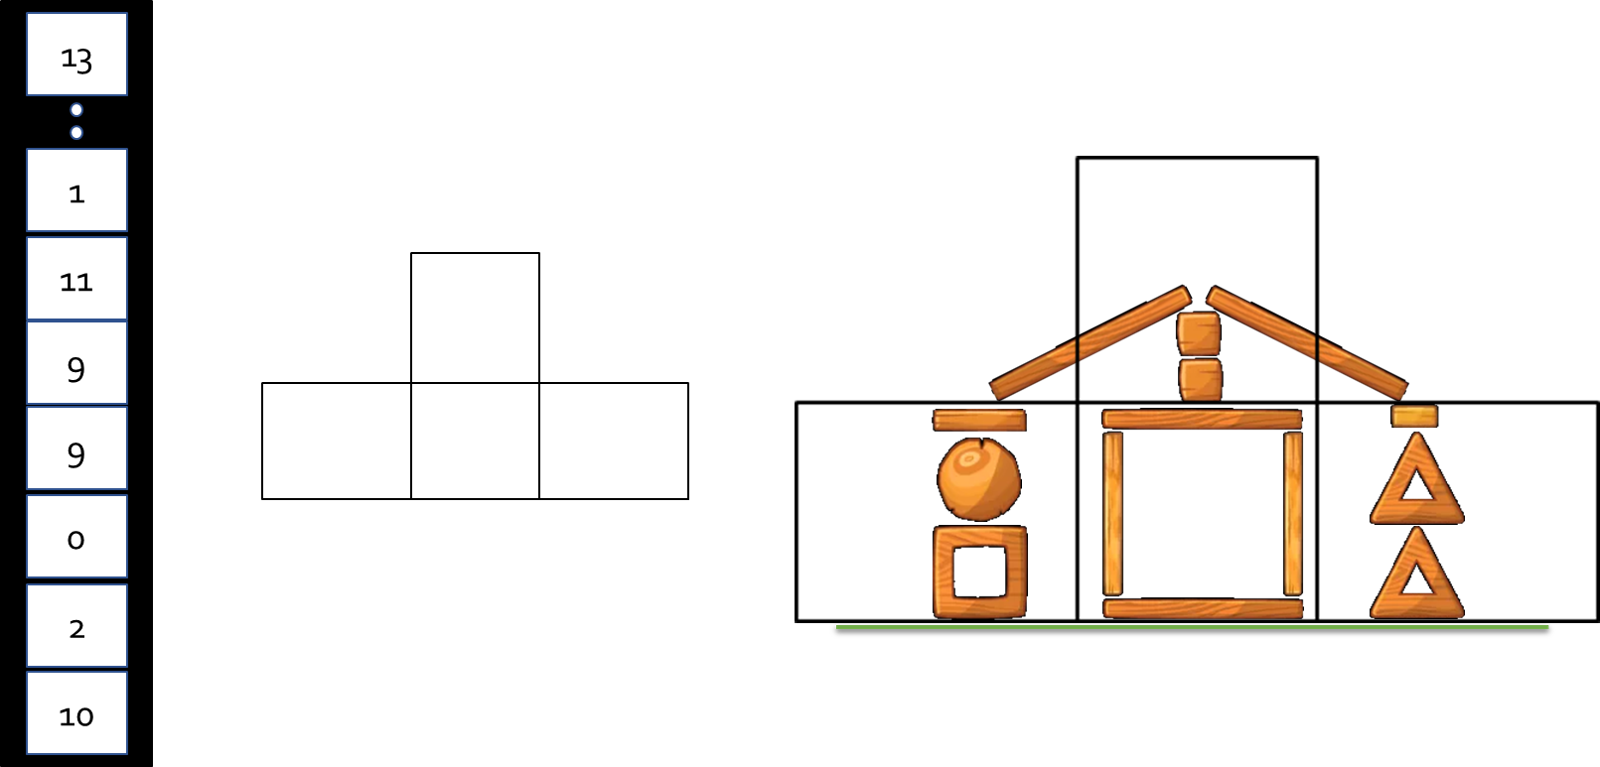
\includegraphics[width=1.0\textwidth]{img/chromosome_thirds.png}
  \caption{Ejemplo del uso de la regla de tercios en un conjunto de piezas, el cromosoma de un individuo(izquierda) se combina con la máscara(centro) para generar una estructura más compleja(derecha)}
  \label{figure:ruleofthird_on_pieces}
\end{figure}

\begin{figure}
  \centering
  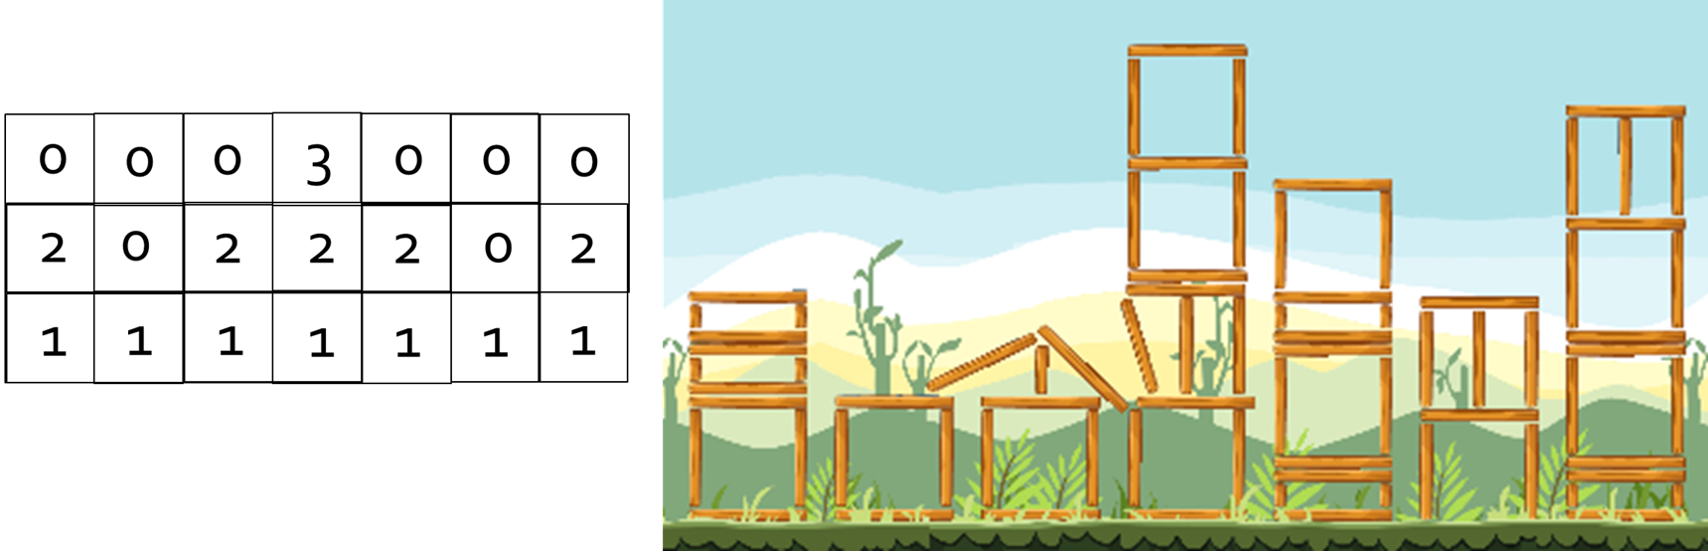
\includegraphics[width=1.0\textwidth]{img/result_example_thirds.png}
  \caption{Resultado obtenido utilizando la regla de tercios, la máscara(izquierda) utilizada y el resultado generado(derecha)}
  \label{figure:ruleofthird_on_chromosome}
\end{figure}


